\section{Introduction}
\label{sec:Introduction}

\newcommand{\firstUseGoal}[1]
  %% {\emph{#1}}
  %% {\textbf{#1}}
  {\textbf{\emph{#1}}}

%%%%%%%%%%%%%%%%%%%%%%%%%%%%%%%%%%%%%%%%%%%%%%%%%%%%%%%%%%%%%%%%%%%%%%%%%%%%%%%%
%% \rkc{Part 1.1: Motivation and SAL/CAL/FPF. Editing TBD.}

In most programming contexts, the design of data structures and algorithms is chiefly focused on performance, but in \emph{dependently-typed proof assistants}, evaluation performance is often unimportant since checking a proof requires type-checking but not actual evaluation.
%
As such, proof assistants often use entirely different data structures than those of conventional settings, with a focus on simplicity or useful proof-theoretic properties.

This paper considers the implementation of \emph{dictionaries}, \ie{} finite mappings from keys to values.
%
The dictionary is a fundamental utility in most programming contexts and serves a broad range of purposes, so the choice of implementation is very important.
%
In conventional languages, dictionaries are implemented with auto-balanced trees or hashtables, which are highly performant, but also very complicated.
%
This paper discusses four alternatives ---three conventional and one novel--- that are often better suited to proof development.

\subsection{Background}

This paper assumes familiarity with statically typed functional languages (\eg{} Haskell, OCaml), and relevant concepts such as Hindley-Milner type systems, pattern-matching, data types, and product types.
%
A cursory background on \emph{proof assistants} and \emph{dependent types} is developed during the course of this introduction, but unfamiliar readers are encouraged to review a more thorough treatment such as \citep{plfa} or \citep{Pierce:SF1}.

A \emph{proof assistant} is a programming language with first-class support for defining and proving theorems, together with editor tools that ease the development of proofs.
%
Many popular proof languages, including Coq and Agda, are founded on \emph{dependent types}, in which a type can be parameterized by concrete values such as numbers, lists, or functions,
%
and in which theorems are types, proofs are functions (or other concrete values), and type checking subsumes proof checking.

\subsection{Conventional Solutions and their Limitations}

\begin{teaserfigure}
\centering
%% \begin{figure*}
\newcommand{\lameq}[1]{$\lambda x$. $x = {#1}$}
\begin{tabular}{ l l }
 %% \Sal{} (\SAL) & [(3, "c"), (1, "b"), {\color{gray} (3, "q")}, (6, "d")] \\
 \Sal{} & [(3, "c"), (1, "b"), {\color{gray} (3, "q")}, (6, "d")] \\
 \Cal{} & [(1, "b"), (3, "c"), (6, "d")] \\ %% \quad (insert function dedupes and preserves canonical order)
 \Fpf{} & \lameq{3} ? "c" : (\lameq{1} ? "b" : (\lameq{3} ? {\color{gray} "q"} : (\lameq{6} ? "d" : $\bot$) $x$) $x$) $x$ \\
 %% \Fpfk{} & ((\lameq{3} ? "c" : (\lameq{1} ? "b" : (\lameq{3} ? {\color{gray} "q"} : (\lameq{6} ? "d" : $\bot$) $x$) $x$) $x$), [1, 3, 6])  \\
 \Dd{}  & [(1, "b"), (1, "c"), (2, "d")]
\end{tabular}
%% \caption{Dictionary representations which result from adding the sequence of keys 6, 3, 1, and 3 (again).}
%
%% \captionsetup{justification=centering}
%% \caption{Dictionary representations after mapping the sequence of keys 6, 3, 1, and 3 (again). \\
%% Each represents the same finite map: %% TODO macros if/when this stabilizes
%% \{ $1 \mapsto ``b"$, $3 \mapsto ``c"$, $6 \mapsto ``d"$ \}
%% }
%
\caption{Dictionary representations after inserting the sequence of keys 6, 3, 1, and 3:
\{ $1 \mapsto ``b"$, $3 \mapsto ``c"$, $6 \mapsto ``d"$ \}
}
%
\label{fig:intro-example}
%% \end{figure*}
\vspace{0.15in} %% SPACE HACK: between teaser figure and Abstract
%% \vspace{0.05in} %% SPACE HACK: between teaser figure and Abstract
\end{teaserfigure}


\subsubsection{\Sal{}s}

The simplest representation for a dictionary, an \emph{\sal}, is merely a list of key-value pairs~\citep[Lists]{Pierce:SF1}.
%
Insertion and destruction are trivially achieved by the cons operator (\texttt{::}) and pattern matching, respectively.
%
Lookup is only slightly more involved:
%
\begin{lstlisting}
  -- assumes that the key type K is fixed
  -- $\forall${V} is an implicit type parameter
  assoc-list-lookup : $\forall${V} $\rightarrow$ List (K $\times$ V) $\rightarrow$ K $\rightarrow$ Maybe V
  assoc-list-lookup [] _ = None
  assoc-list-lookup ((k1 , v1) :: l) k =
    with eq-dec-K k k1                 -- 'eq-dec-K k k1' checks whether k == k1 ...
  ... | Inl _ = Some v1                -- if k == k1, then 'eq-dec-K k k1' evals to 'Inl _'
  ... | Inr _ = assoc-list-lookup l k  -- otherwise, 'eq-dec-K k k1' evals to 'Inr _'
\end{lstlisting}

\parahead{Limitation: Lack of \Extensional}

Though easy to work with and reason about, \sal{}s have a drawback which can cause difficulty during proof development:
%
because they allow duplicate bindings for the same key and they are sensitive to the order of insertions, many distinct \sal{}s represent the same semantic mapping.
%
For example, the first two lines of \autoref{fig:intro-example}
%
show two distinct association lists (among others) that represent a dictionary with three particular bindings.
%
In other words, \sal{}s lack \firstUseGoal{\Extensional}: the property that any two non-identical valid lists must have distinct semantic meanings.
%
\Extensional{} can make proofs easier ~\cite[Maps]{Pierce:SF1} and permits the use of the built-in equality proposition to establish semantic equivalence.
%

Proof languages such as Agda have built-in support for \emph{reflexive equality}, which judges two values (of the same type) as being equal if and only if they are precisely identical:
\begin{lstlisting}
  -- In Agda, 'Set' is (roughly) the type of all types (incl. propositions).
  -- _==_ means that == is infix and binary.
  -- The first explicit arg is named x and is of type T,
  -- the second explicit arg is also of type T but is unnamed.
  -- Because == is a proposition, the "return type" is Set.
  data _==_ {T : Set} (x : T) : T $\rightarrow$ Set where
    -- A constructor of a proposition is a proof of that proposition.
    -- refl is the only constructor - for any x, refl is a proof that x == x.
    refl : x == x
    -- There's no way to establish equality of two arbitrary values x and y.
\end{lstlisting}

The built-in equality proposition is a common and intuitive way to judge the equality of two values.
%
Furthermore, proof assistants have special features for working with it, which can be harnessed to simplify and expedite proof development.
%
As such, it's very useful to be able to use this proposition, rather than to define a custom proposition that judges the semantic equivalence of two dictionaries.
%
\autoref{sec:CaseStudy} and \autoref{sec:Discussion:Generality} further demonstrate the importance of \Extensional{} by showing that its absence can render some theorems, such as the important \emph{structural properties} \emph{contraction} and \emph{exchange}~\citep{StructProp}, false.

%% %% \begin{figure}[b]
\begin{figure}[h]
  \centering
  \begin{tikzpicture}[nodes = {align = left}]
    %% \node [scale=.45]
    \node [scale=.33]
    {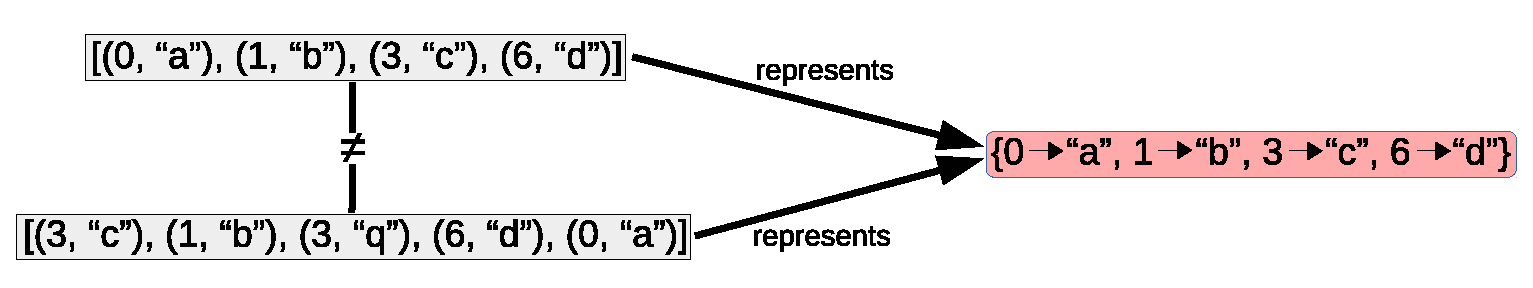
\includegraphics{figs/unequal.eps}};
  \end{tikzpicture}
  \caption{Two distinct \sal{}s representing the same semantic mapping. \rkc{Let's show the first two rows from Fig 1. And let's fit this into one column.}}
  \label{fig:uneq}
\end{figure}


\subsubsection{\Cal{}s}

To establish a one-to-one correspondence between association lists and semantic mappings, and thus \Extensional, one solution~\citep{FMapList} is to maintain a \emph{canonical}
%
form that is semantically valid and unique, namely, a list in which there are no duplicate keys and, furthermore, where keys are in sorted order.%
%
\footnote{\hspace{0.01in}%
%
The Coq standard library~\citep{FMapInterface}, describes unordered but deduplicated \sal{}s as ``weak,'' implying that \cal{}s are ``strong.''
%
}
%
The second association list shown in \autoref{fig:intro-example} is one such example.
%
This approach requires a more sophisticated \texttt{insert} function than that of the naive \sal{} approach:
\begin{lstlisting}
  -- assumes that the key type K is fixed
  cal-insert : $\forall${V} $\rightarrow$ List (K $\times$ V) $\rightarrow$ (K $\times$ V) $\rightarrow$ List (K $\times$ V)
  cal-insert [] (k , v) = (k , v) :: []
  cal-insert ((k1 , v1) :: l) (k , v) =
    with ord-dec-K k k1
  ... | Inl _       = (k , v) :: (k1 , v1) :: l         -- k < k1
  ... | Inr (Inl _) = (k , v) :: l                      -- k == k1
  ... | Inr (Inr _) = (k1 , v1) :: cal-insert l (k , v) -- k > k1
\end{lstlisting}

\parahead{Limitation: Lack of \SemTot}

Although the \cal{} approach is \extensional, it has another drawback; the list-of-pairs type allows arbitrary, possibly invalid lists, so each \cal{} must be packaged with a proof of validity:
\begin{lstlisting}
  -- assumes that the key type K is fixed
  data _valid-cal $\forall${V} (List (K $\times$ V)) : Set
    EmptyVal  : [] valid-cal
    SingleVal : $\forall${k v} $\rightarrow$ ((k , v) :: []) valid-cal
    -- For any k1, k2, v1, v2, and l, if k1 < k2, and (k2 , v2) :: l is valid,
    -- then ManyVal stands as a proof that (k1 , v1) :: (k2 , v2) :: l is valid.
    ManyVal   : $\forall${k1 k2 v1 v2 l} $\rightarrow$
                  k1 < k2 $\rightarrow$
                  ((k2 , v2) :: l) valid-cal $\rightarrow$
                  ((k1 , v1) :: (k2 , v2) :: l) valid-cal

  cal : $\forall${V} $\rightarrow$ Set
  -- '$\sum$[ x $\in$ T ] (p x)' packages x (of type T) with a proof that it satisfies p
  cal {V} = $\sum$[ l $\in$ List (K $\times$ V) ] (l valid-cal)
\end{lstlisting}

This paper coins the term \firstUseGoal{\semanticallyTotal} to describe any data structure whose type is free of proof terms and yet contains no invalid members ---
%
\ie{} the mapping from values in the underlying type to their semantic meanings is total.
%
To illustrate, a pair of integers is not a \semanticallyTotal{} data structure for the rational numbers, since if the second integer is $0$ then the pair is invalid,
%
but a pair of an integer and a natural, where the natural represents the denominator minus $1$, \emph{is} \semanticallyTotal{} (note that neither of these data structures is \extensional).
%
The downsides of having to use validity proofs are discussed in \autoref{sec:CaseStudy} and \autoref{sec:Discussion:Generality}.

\subsubsection{\Fpf{}s}

A third conventional solution is to represent dictionaries as finite partial functions~\cite[Maps]{Pierce:SF1} (\ie{} functions that return \texttt{None} for all but finitely many inputs).
%
The third line of \autoref{fig:intro-example} depicts a nested $\lambda$-expression that serves as the ``lookup table'' (we omit the \texttt{Some} constructors for space).
%
This approach can be made \extensional{} by postulating \emph{functional extensionality}~\mbox{\cite[Logic]{Pierce:SF1}}, which axiomatically asserts that $(\forall x, f(x) == g(x)) \Rightarrow f == g$.
%
On the other hand, this approach technically fails to satisfy \SemTot, since the function type permits \emph{non-}finite maps.
%
Even so, this is often not a problem in practice --- as long as the dictionary is never iterated, destructed, or counted, an infinite dictionary is indistinguishable from a finite dictionary.
%
Furthermore, a dictionary built from a finite program can only have finitely many mappings.
%
The more serious problems are that, unlike either association list approach, functions lack \firstUseGoal{\DecidableEq} and cannot be \firstUseGoal{\destructed}.

\parahead{Limitation: Lack of \DecidableEq}

While a proof that $x == y$ establishes the truth that $x$ and $y$ are equal, the \texttt{==} proposition is not capable of \emph{deciding} whether or not two arbitrary values are equal.
%
To \emph{decide} this question, we need to define a function that accepts two arguments (of the same type) and returns either a proof that they are equal or a proof that they are not equal:
\begin{lstlisting}
  -- 'P $\rightarrow \bot$' means that P is false.
  eq-dec-K : (x y : K) $\rightarrow$ ((x == y) $\lor$ (x == y $\rightarrow \bot$))
  eq-dec-K x y = ?  --  the implementation will depend on the type K
\end{lstlisting}

Note that proof languages like Coq and Agda are \emph{constructive}; they elide the \emph{law of the excluded middle}, so it's possible for a proposition to be neither provably true nor provably false.
%
As such, the ability to decide whether some proposition (such as the equality of two values) is true or false cannot be taken for granted --- if this ability is needed, it must be explicitly established by defining a function such as the one above.
%
In the case of functions, it's not possible to establish that two arbitrary functions are unequal, so there is no way to establish decidability.
%
Naturally, deciding whether or not two dictionaries are equal is important and useful for many of the same reasons it would be in a more conventional language, so the lack of \DecidableEq{} is a substantial weakness.

\parahead{Limitation: Lack of Destructibility}

The inability to destruct a function is more intuitive --- destruction is essentially the same as in other functional languages, where pattern-matching is typically used to separate one element of a collection (often the \emph{head}) from the rest of the collection.
%
A lambda value can't be destructed or picked apart in any way, so its values also can't be iterated or counted.
%
The function could be packaged with a set indicating its domain --- \ie{}~a canonical list of keys --- but would then have to include a proof that those keys are correct, violating \SemTot{} in the same troublesome way that \cal{}s do.

\subsection{Core Properties}

In some cases, the aforementioned drawbacks are minor or can be worked around.
%
But developing large proofs is challenging, so any stumbling block can cause exorbitant increases in verbosity, time, effort, and accidental complexity.
%
Furthermore, as shown in \autoref{sec:CaseStudy}, there are cases where these drawbacks make a proof task not merely difficult, but outright impossible.

%%%%%%%%%%%%%%%%%%%%%%%%%%%%%%%%%%%%%%%%%%%%%%%%%%%%%%%%%%%%%%%%%%%%%%%%%%%%%%%%
%% \rkc{Part 1.2: Summary of Design Goals. Editing TBD.}

Ideally, when working in a proof assistant, an implementation of a data structure---dictionaries in particular for this paper---would satisfy the following properties:

\newcommand{\designGoal}[1]
  {\textbf{\emph{#1:}}}

\begin{enumerate}

\item
%
\designGoal{\SemTot}
%
Every value in the representation type is semantically valid, \ie{}~the mapping from values to their semantic meanings is total.

\item
%
\designGoal{\SemInj}
%
Built-in equality corresponds to semantic equivalence, \ie{} two unequal values have different semantic meanings.

\item
%
\designGoal{\EqDec}
%
Built-in equality is decidable for the representation type.

\end{enumerate}

Furthermore, in addition to properties about the external interface of the data structure, it is often useful to retain the ability to inspect, iterate, and manipulate sub-dictionaries.
%
%% Thus, our final design goal:

\begin{enumerate}

\item[(4)]
%
\designGoal{\EzDstr}
%
The ability to decompose a data structure into atomic subparts in a convenient manner.

%% to facilitate

%% sufficiently

\end{enumerate}

\newcommand{\no}
  %% {No}
  %% {}
  {\color{lightgray}\phantom{$^*$}\xmark\phantom{$^*$}}
\newcommand{\noIO}
  %% {\color{lightgray}\phantom{$^*$}\xmark$^*$}
  {{\color{lightgray}\phantom{$^*$}\xmark}\footnotemark[3]} % 3 is hard-coded, but I see no other way
\newcommand{\yes}
  %% {Yes}
  %% {\phantom{*}\cmark\phantom{*}}
  {\phantom{$^-$}\cmark\phantom{$^-$}}
\newcommand{\yesMinus}
  %% {Yes*}
  %% {\phantom{*}\cmark*}
  {\phantom{$^-$}\cmark$^-$}
\newcommand{\yesPlus}
  %% {Yes*}
  %% {\phantom{*}\cmark*}
  {\phantom{$^-$}\cmark$^+$}
\newcommand{\eq}
  %% {Decidable equality}
  %% {Eq K}
  %% {(=) : (K,K) -> Bool}
  {$(=)$}
\newcommand{\ord}
  %% {Orderable}
  %% {Eq K, Ord K}
  %% {(=),(<) : (K,K) -> Bool}
  {$(=), (<)$}
\newcommand{\isoNat}
  %% {Bijects to naturals}
  %% {K $\leftrightarrow$ Nat}
  {$f\hspace{0.02in}\!:\!\hspace{0.02in}K \leftrightarrow \textit{Nat}$}

\newcommand{\header}[1]
  {\makebox[0.67in]{#1}}
\newcommand{\headers}[6]
  {&\header{#1}&\header{#2}&\header{#3}&\header{#4}&\header{#5}&\header{#6}}

%% \begin{figure}[H]
\begin{figure*}[t]
  \begin{tabular}{ l || c | c | c | c | c || c}
  \multirow{2}{*}{}
           & \multicolumn{5}{c||}{\footnotesize Client Usage}
           & {\footnotesize Implementation} \\ \cline{2-7}
   \headers{\total}{\extensional}{\decidable}{\destructible}{Key Type $K$}{Simple}    \\ \hline
   \Sal    & \yes   & \no        & \yes      & \yes         & \eq       & \yesPlus  \\ %% \hline
   \Cal    & \no    & \yes       & \yes      & \yes         & \ord      & \yesMinus \\ %% \hline
   \Fpf    & \noIO  & \yes       & \no       & \no          & \eq       & \yes      \\ \hline
   %% \Fpfk   & \no    & \yes       & \yes      & \yes         & \ord      & \simple     \\ \hline
   \Dd     & \yes   & \yes       & \yes      & \yesMinus    & \isoNat   & \no
  \end{tabular}
  \caption{Properties of dictionary representations.}
  \label{fig:prop-summary}
\end{figure*}
%% \end{figure}

\footnotetext{\hspace{0.01in}%
%
As aformentioned, this is often not a problem in practice, so for many practical intents and purposes, this may as well be a \cmark.
%
}

\autoref{fig:prop-summary} summarizes the preceding discussion along these dimensions; note that the association list representations can be easily destructed, but destruction is not possible for \fpf{}s.
%
None of the conventional approaches satisfies both \SemTot{} and \SemInj{}, nor more than three of the four properties.

\subsection{Novel Solution: Delta Dictionaries}
%
The four core properties can be (mostly) satisfied by way of \emph{\dds{}} --- although destructible, \EzDstr{} is not fully achieved because destruction of \dds{} is awkward.
%
%% A \dd{} is similar to a canonical association list, but instead of storing each literal key value, it stores the \emph{difference} from the previous key, minus 1.
%
A \dd{} can be described as a ``canonical-by-construction'' association list: instead of storing each literal key value, it stores the \emph{difference} from the previous key, minus 1 (details in \autoref{sec:DD}).
%
For example, compare the canonical association list and \dd{} in \autoref{fig:intro-example}:

\vsepRule

%% keep this in sync with Figure 1
\begin{tabular}{ l l }
 \Cal{} & [(1, \str{a}), (3, \str{b}), (6, \str{c})] \\
 \Dd{}  & [(1, \str{a}), (1, \str{b}), (2, \str{c})]
\end{tabular}

\vsepRule

Every well-typed list-of-pairs is a valid \dd{}, thus no proof term is needed to establish validity (\SemTot).
%
Every unique \dd{} represents a unique semantic mapping, thus built-in equality may be used for semantic equivalence (\SemInj).
%
%% there is a bijection between \dd{} terms and finite maps,
%
Furthermore, we define a function which determines whether or not two \dds{} are equal (\EqDec), and a \texttt{destruct} function, which permits destruction albeit in a more awkward manner than standard pattern matching.

As summarized in \autoref{fig:prop-summary}, delta dictionaries strike a new balance in this design space.
%
Compared to \cal{}s, \dds{} enjoy \SemTot{}---the lone property among those we identify which the \cal{} does not.
%
However, destruction and iteration for \dds{} is substantially more difficult.
%
Furthermore, unlike all of the conventional approaches, \dds{} require a bijection to the naturals, not merely decidable equality or ordering, for their key types.
%
%% Our definition and implementation uses natural numbers for keys, and we illustrate how to use bijections to the naturals as a way of supporting strings, integers, or other key types that can be bijected to the naturals without great difficulty.
%
Lastly, though not a concern from a client's perspective, the implementation of delta dictionaries is considerably more involved than the conventional approaches.

\subsection{Outline}
%
Next, we describe the core operations for delta dictionaries and the relevant metatheory in \autoref{sec:DD}.
%
In \autoref{sec:CaseStudy}, we describe a small case study in proof development that demonstrates the necessity of delta dictionaries.
%
Finally, we conclude in \autoref{sec:Discussion} with a discussion. %% of related work.
%
%% Our implementation and proofs are formalized in Agda and available in the anonymous supplementary materials.
